\subsection{Electronics}
The custom rotator is controlled by a raspberry pi, extended by a custom raspberry pi hat. The hat provides functionallity to read the safty swiches, communicate to two independet magnetic encoder, drive both motors, as well as monitor the motors speed with a quadrature encoder. The Hat also features a EEPROM, which is specified by the raspberry pi foundation, to call it an 'offical' pi hat. The pi and both motors are powered through an of the shelf power over ethernet (poe) adapter.

\subsubsection{choice of electronics}
We had a working prototype within the first couple of weeks, which enabled us to test lots of feature early on. In the beginning, we needed three cables to power the raspberry pi, the motors, as well as to provide a data cable for communication. The power over ethernet adapter allowed us to only have one cable and simplify the design.
To move away from our orignal breadboard design connected to some of the shelfs components, we also designed our own raspberry pi hat.


\subsubsection{how to connect, pinout}
\begin{figure}[h]
	\centering
	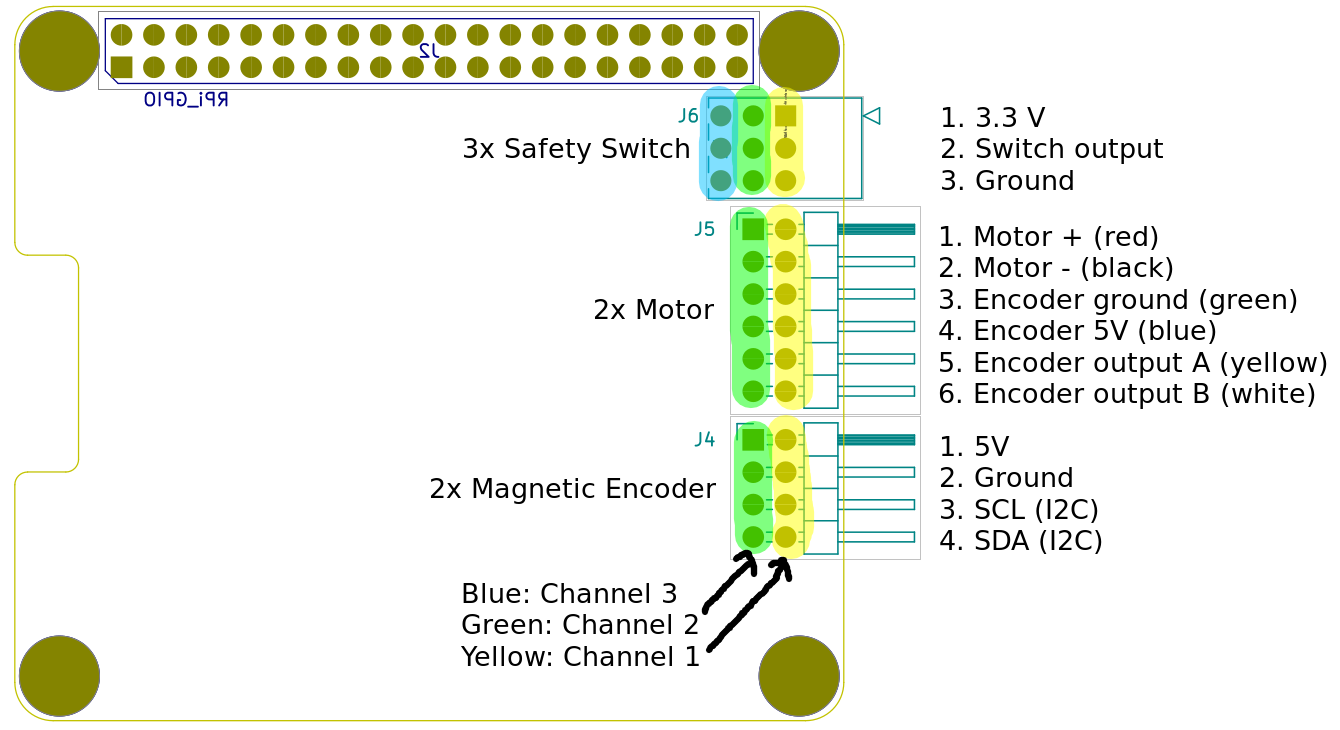
\includegraphics[width=\linewidth]{../art/PCB Pinout.png}
	\caption{Raspberry pi hat pinout}
\end{figure}

\subsubsection{Electronic Design}


\begin{figure}[h]
	\centering
	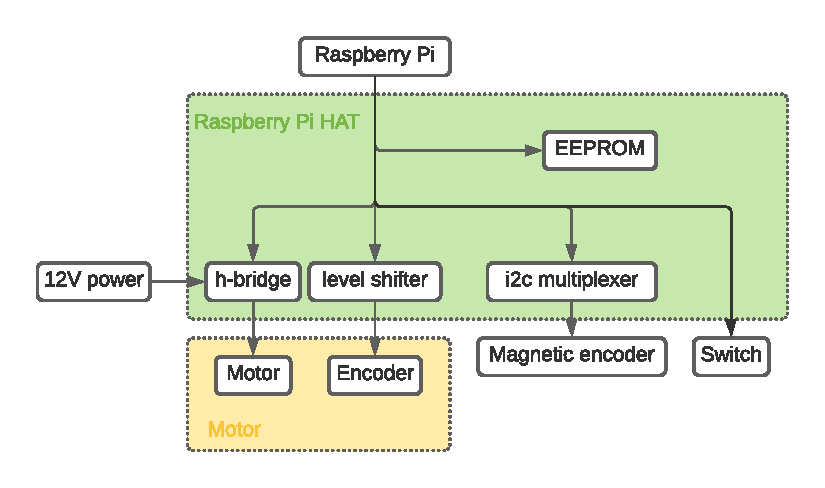
\includegraphics[width=\linewidth]{../art/PCB Block diagram.pdf}
	\caption{Raspberry pi HAT blockdiagramm}
\end{figure}

\begin{figure}[h]
	\centering
	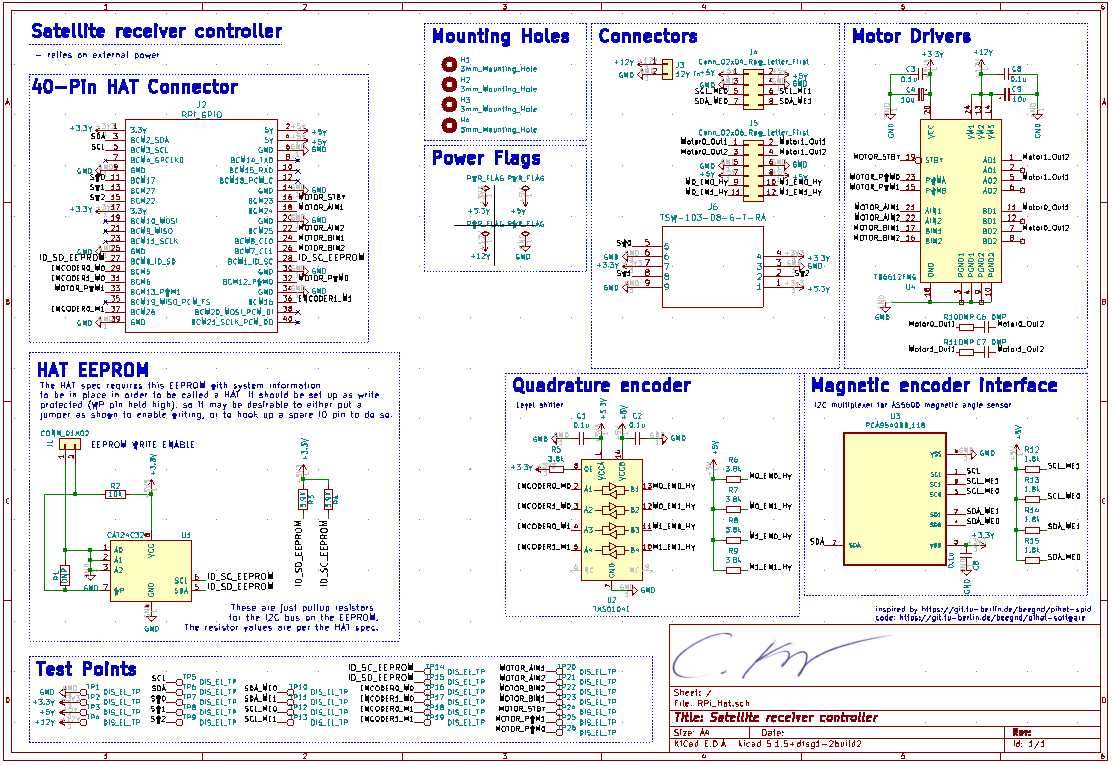
\includegraphics[width=\linewidth]{../art/pcbSchematic.png}
	\caption{Schematic of Raspberry Pi hat}
\end{figure}


\begin{figure}[h]
	\centering
	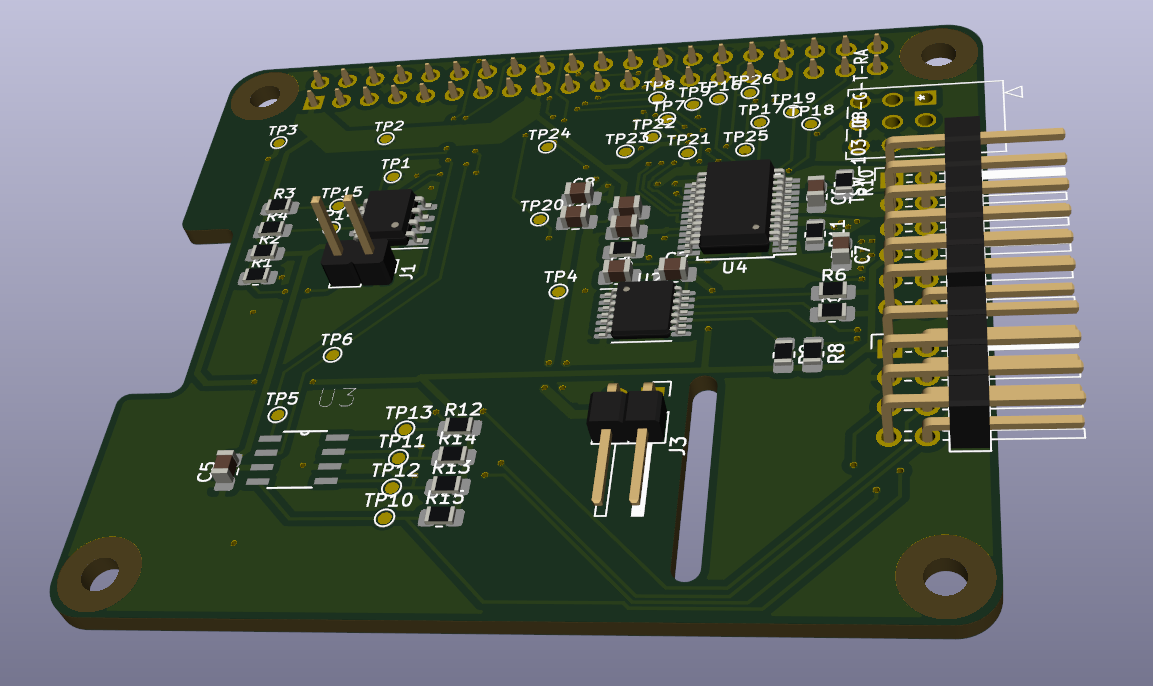
\includegraphics[width=\linewidth]{../art/PCB.png}
	\caption{PCB of Raspberry Pi hat}
\end{figure}


\begin{figure}[h]
	\centering
	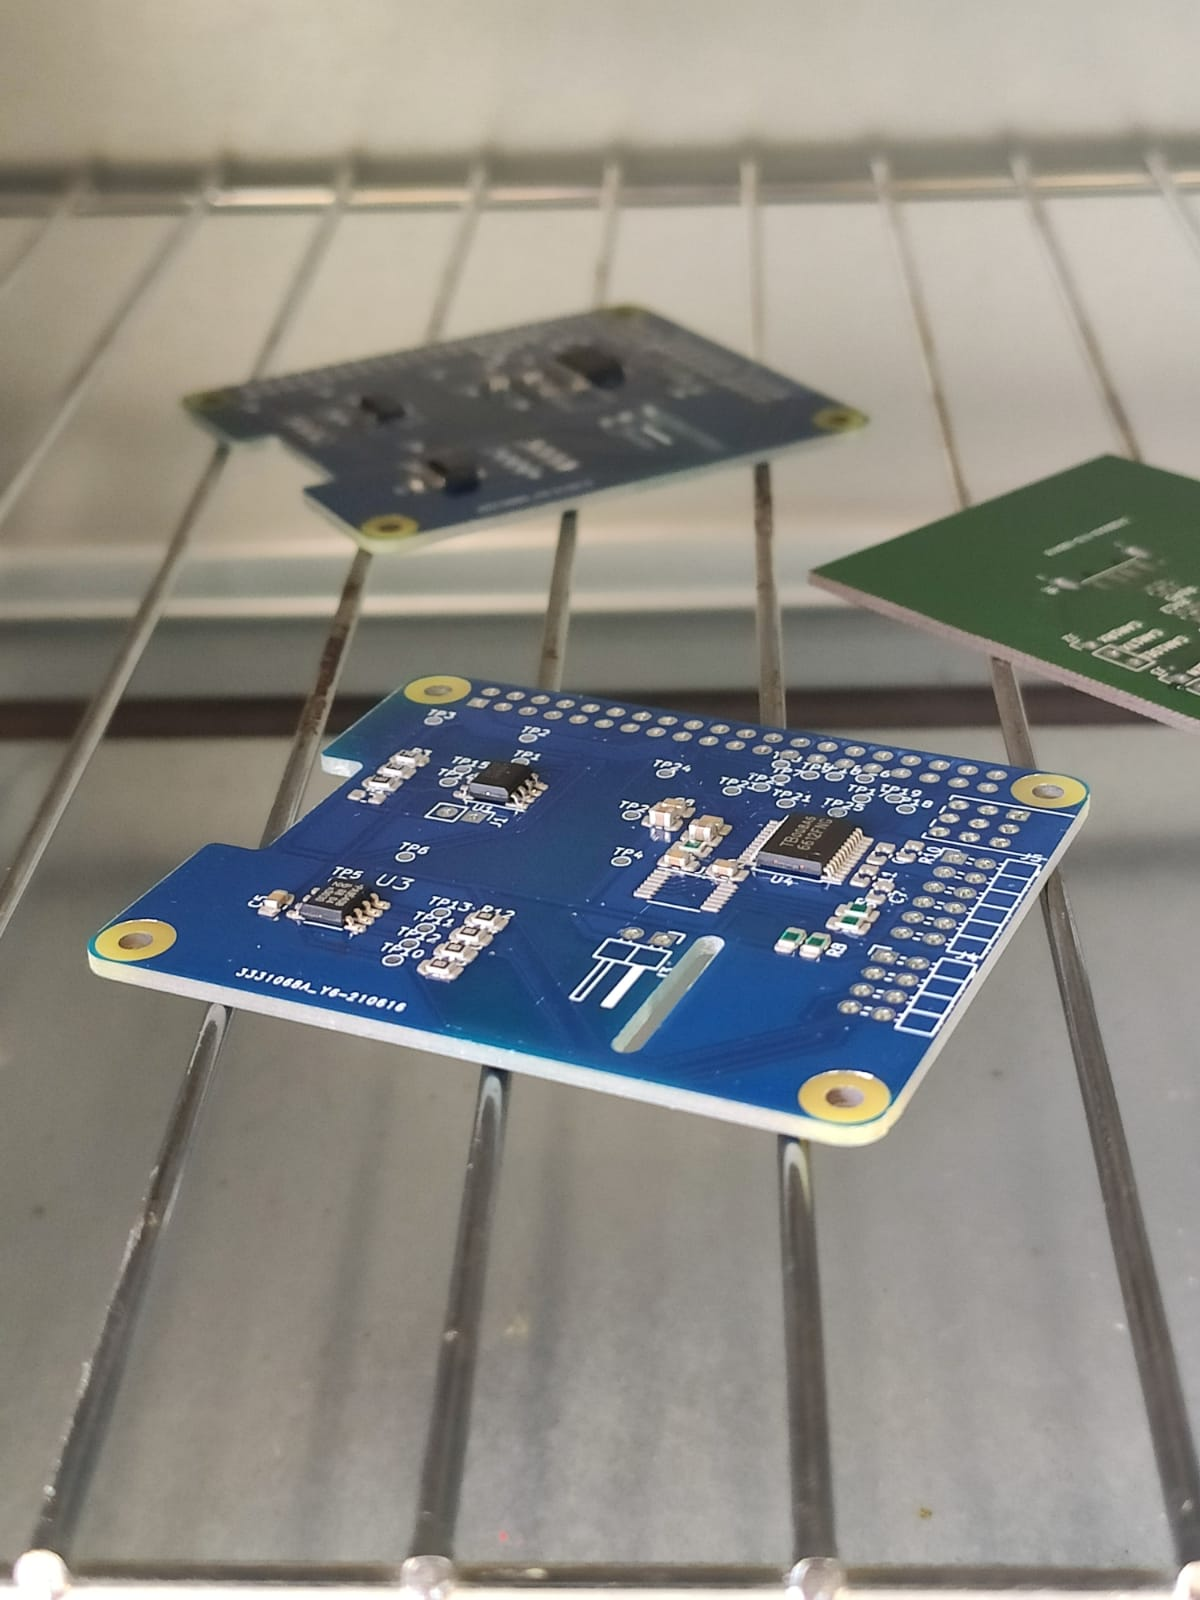
\includegraphics[width=\linewidth]{../art/pcb Manufactureing.jpeg}
	\caption{Raspberry pi manufacturing}
\end{figure}


\subsubsection{fabrication and rework}